\label{ordernsquared}
Elementary sorts are also referred to as $O(N^2)$ sorts. This is due to the
manner in which they check every key in the array in order to sort a single key;
for every key to be sorted, every other key is checked.  Four of these sorts are
discussed here: insertion sort, selection sort, bubblesort and shakersort,
along with improved versions of bubblesort and shakersort.

\section{Selection Sort}

Selection sort works in a straightforward manner. It begins by 
searching the unsorted array for the smallest key, then swapping it into the
first position in the array. This key is now the first element of a sorted
array, being built from the left. The remainder of the array is
still unsorted, and it is now searched for its smallest key, which is swapped
into place. This continues until the entire array is sorted. Sample code is in
Figure \vref{Selection sort code}.

\code{Selection sort code}{selectsort.c}
\subsection{Testing}
%TESTING
All elementary sorts are only sorted up to 65536 keys in the simulations, and
262144 keys with the performance counters. Due to the quadratic nature of
these sorts, days and weeks would be required to run tests on the larger arrays.

\subsubsection{Expected Performance}
Sedgewick provides a discussion on the performance of elementary sorts. The
observations on instruction count are his, and come from \cite{Sedgewick02}.

Selection sort uses approximately $N^2/2$ comparisons and exactly $N$ exchanges.
As a result, selection sort can be very useful for sorts involving very large
records, and small keys. In this case, the cost of swapping keys dominates the
cost of comparing them. Conversely, for large keys with small records, the cost
of selection sort may be higher than for other simple sorts.

The performance of selection sort is not affected by input, so the instruction
count varies very little.  Its cache behaviour is also not affected by input,
and selection sort performs very badly from a cache perspective. There are $N$
traversals of the array, leading to bad temporal reuse. If the array doesn't fit
inside the cache, then there will be no temporal reuse.

The level 1 cache should have bad performance as a result. Since it is smaller
than the array, the performance of the level 1 cache should simulate the
performance of the level 2 cache.

\label{selection branches logn}
The branch prediction performance is not expected to be bad. Flow
control predictions are very straightforward, and should result in
very few misses.  Comparison predictions, however, are very
numerous. Each traversal of the array has an average of $N/2$
comparisons, as we search for the smallest key in the unsorted part of
the array. During the search, the algorithm compares each key with the
smallest key seen so far. In a random array, we would expect that the
candidate for the smallest key (the left-to-right minimum) would
change frequently towards the start of the array, making the
comparison branch rather unpredictable. However, as the traversal
continues, the left-to-right minimum will become smaller, and thus
more difficult to displace. It will become very unusual to find a
smaller key, and thus the branch will almost always resolve in the
same direction.  Therefore, the comparison branch will quickly become
very predictable.

Knuth \cite{Knuth97} analyses the number of changes to the
left-to-right minimum when searching for the minimum element of an
array. He shows that for $N$ elements, the number of changes is $H_N -
1$, where $H_N$ is the harmonic series:

$$H_N = 1 + \frac{1}{2} + \frac{1}{3} + ... + \frac{1}{N} =  \sum_{k=1}^{N}
\frac{1}{k},  \hspace{0.4cm}  N \geq 1$$

Within practical sorting ranges, $H_N$ grows at a rate similar to
$log(N)$. Thus, in the average case, we can expect that the comparison
branch will mostly go in the same direction, making the branch highly
predictable.

Knuth also presents the number of changes to the left-to-right minimum
in the best case (0 changes) and worst cases ($N-1$ changes).  In the
worst case, the array is sorted in reverse order, and so the
left-to-right minimum changes on every element. Interestingly, the
worst cases for the number of changes is not the worst case for branch
mispredictions. If the minimum changes for every element, then the
comparison branch will always resolve in the same direction, and thus
be almost perfectly predictable.  From the point of view of branch
prediction, frequent changes (preferably with no simple pattern) are
the main indicator of poor performance, rather than the absolute
number of times that the branch resolves in each direction. The worst
case for selection sort would probably be an array which is partially
sorted in reverse order --- the left-to-right minimum would change
frequently, but not predictably so.


\section{Insertion Sort}

Insertion sort, as its name suggests, is used to insert a single key into its
correct position in a sorted list. Beginning with a sorted array of length one,
the key to the right of the sorted array is swapped down the array a key at a
time, until it is in its correct position. The entire array is sorted in this
manner.

An important improvement to insertion sort is the removal of a bounds check. In
the case that the key being sorted into the array is smaller than the smallest
key in the array, then it will be swapped off the end of the array, and continue
into the void. To prevent this, a bounds check must be put in place, which will
be checked every comparison, doubling the number of branches and severely
increasing the number of instructions. However this can be avoided by using a
sentinel. This is done by finding the smallest key at the start, and putting it
into place. Then no other key can be smaller, and it will not be possible to
exceed the bounds of the array. Another technique would be to put $0$ as the
smallest key, storing the key currently in that position, then putting it in
place at the end. This would use a different insertion sort, with a bounds
check, going in the opposite direction. The first of these is shown in the
sample code in Figure \vref{Insertion sort code}.

\code{Insertion sort code}{insertsort.c}
\subsection{Testing}
\subsubsection{Expected Performance}
These instruction count observations are again due to Sedgewick.  Insertion sort
performs in linear time on a sorted list, or slightly unsorted list. With a
random list, there are, on average, there are $N^2/4$ comparisons and $N^2/4$
half-exchanges\footnote{A half-exchange is where only one part of the swap is
completed, with the other value stored in a temporary to be put in place later.}.
As a result, the instruction count should be high, though it is expected to be
lower than selection sort.

The cache performance should be similar to selection sort as well. While
selection sort slowly decreases the size of the array to be considered,
insertion sort gradually increases the size. However, each key is not checked
with every iteration. Instead, on average, only half of the array will be
checked, and there will be high temporal and spatial reuse due to the order in
which the keys are accessed. This should result in lower cache misses than
selection sort.

The flow control of insertion sort is determined by an outer loop, which should
be predictable, and an inner loop, which, unlike selection sort, is dependent on
data. As a result, the predictability of the flow control is highly dependant on
the predictability of the comparisons.

\section{Bubblesort}
Bubblesort, as its name suggests, works by bubbling small keys from right of
the array to the left. It begins by taking a key from the end and moving it left
while it is less than any keys it passes. Once it comes across a smaller key, it
changes to this key, and moves it towards the left of the array. In this way, every
iteration the smallest key moves left to its final position, and other small
keys are slowly moved left, so that the unsorted part of the array becomes more
sorted as bubble sort continues.

An improvement made to bubblesort is that it stops as soon as the array is
sorted. Sample bubblesort code is in Figure \vref{Bubblesort code}.

\code{Bubblesort code}{bubblesort.c}
\subsection{Testing}
\subsubsection{Expected Performance}
These instruction count observations are again due to Sedgewick.  Bubblesort has
$N^2/2$ comparisons and exchanges. The number of passes over the array, and size
of each pass is the same as selection sort, and similar instruction count
results are expected.  The extra check to see if the array is sorted adds
$O(NlogN)$ instructions, but this is small in comparison to the number of
instructions saved if the sort ended early.

The cache performance of bubblesort should be the same as that of selection
sort. Each key loaded into the cache is used just once, and will be ejected from
the cache if the data set is large enough.

The branch predictive performance is also expected to be similar. While
selection sort has $O(NH_N)$ mispredictions, each of bubblesort's comparisons
has the potential to be a misprediction, and not just in the pathological case.
However, as the sort continues and the array becomes more sorted, the number of
mispredictions should decrease. The number of flow control mispredictions should
be very low.

\section{Improved Bubblesort}
Improved bubblesort incorporates an improvement to end bubblesort early. The
bubblesort implementation described in the previous section ends early if it
detects that the array is fully sorted. It keeps a binary flag to indicate if
there were any exchanges along the way. Instead, improved bubblesort keeps track
of the last exchange made, and starts the next iteration from there. This means
that any pockets of sorted keys are skipped over, not just if they occur at the
end. Improved bubblesort code is shown in Figure \vref{Improved bubblesort
code}.

\code{Improved bubblesort code}{improved_bubblesort.c}
\subsection{Testing}
\subsubsection{Expected Performance}
It is expected that improved bubblesort should perform faster than the original
in all metrics. Instruction count, were there no conditions that allowed keys to
be skipped, would be the similar, since few extra instructions are added. The
flow of the algorithm is the same, though there should be fewer iterations,
especially at the start, when iterations are longer, so cache accesses, and
branch misses should be reduced along with instruction count.

\section{Shakersort}
Shakersort is sometimes called back-bubblesort. It behaves like a bubblesort
which moves in both directions rather than just one way. Both ends of the array
become sorted in this manner, with the larger keys slowly moving right and the
smaller keys moving left. Sample code for shakersort is shown in Figure
\vref{Shakersort code}.

\code{Shakersort code}{shakersort.c}
\subsection{Testing}
\subsubsection{Expected Performance}
The instruction count of shakersort is expected to be exactly the same as
bubblesort, while its cache performance is expected to be superior. A small
amount of temporal reuse occurs at the ends of the array, as each key is used
twice once its loaded into the cache. In addition, when the array is not more
than twice the size of the cache, then the keys in the centre of the array are
not ejected from the cache at all.

Finally, the branch prediction results are expected to be the same as in bubble
sort, with one difference.  Keys which must travel the entire way across the
array are taken care of earlier in the sort. If the largest key is in the
leftmost position, it must be moved the entire way right, which causes misses
for every move in bubblesort, since each move is disjoint from the next. In
shakersort, however, each move in the correct direction will follow a move in the
same direction, each of which should be correctly predicted. This works for a
lot of keys, which are more likely to move in continuous movements than they are
in bubblesort, where only small keys on the right move continuously. The
performance should improve noticeably as a result.

\section{Improved Shakersort}
Improved shakersort incorporates the same improvements over shakersort as
improved bubblesort does over bubblesort, that is, it skips over pockets of
sorted keys in both directions, as well as ending early. The code for improved
shakersort is in Figure \vref{Improved shakersort code}.

\code{Improved shakersort code}{improved_shakersort.c}
\subsection{Testing}
\subsubsection{Expected Performance}
It is expected that the improvements will make shakersort faster in all cases
than its original form.

\section{Simulation Results}

%TODO check that this is put in after the titlepage
%TODO check that the captions are the same as the captions at the end of the
%other chapters
% I'm doing a slightly different result here. Level 2 doesn't interest us, so put
% in 2 prediction results instead - 1 for select/insert, 1 for bubble/shaker
\afterpage{
\label{Elementary sort results}

\thispagestyle{empty}
\clearpage
\enlargethispage{14em}
\vspace*{-8em}
\begin{figure}[H]
\begin{changemargin}
\subfigure[Cycles per key - this was measured on a Pentium 4 using hardware performance counters.]
{\label{elementary cycles}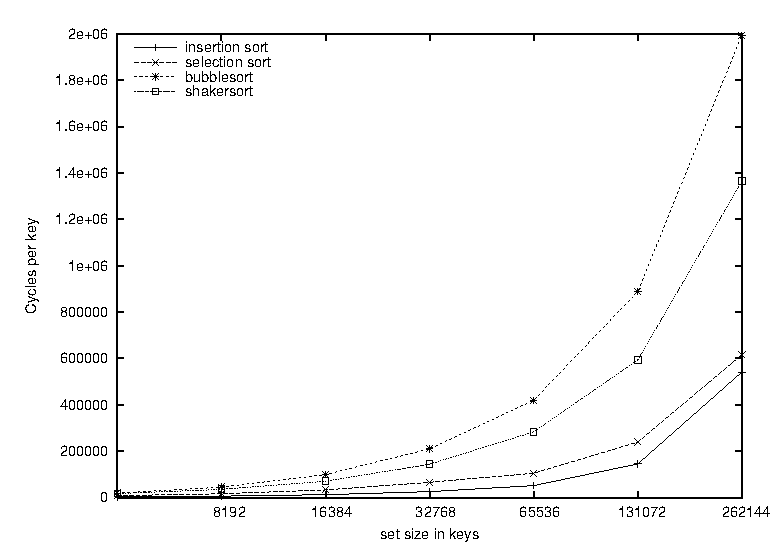
\includegraphics[scale=\myscale]{plots/on2_-_cycles.eps}}
\subfigure[Instructions per key - this was simulated using SimpleScalar \cc{sim-cache}.]	
{\label{elementary instructions}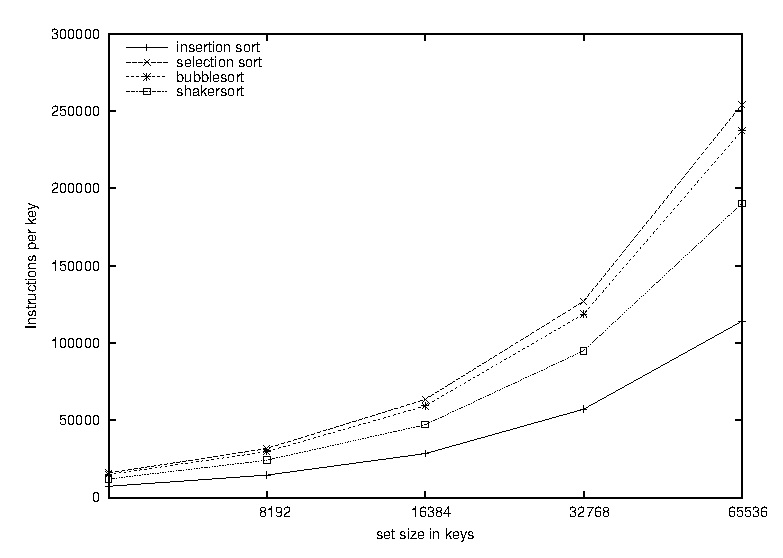
\includegraphics[scale=\myscale]{plots/on2_-_Instructions.eps}}
\end{changemargin}
\vspace*{6em}
\caption{Simulated Instruction count and empiric cycle count for elementary sorts}
\label{Simulated Instruction count and empiric cycle count for elementary sorts}
\end{figure}
\newpage

\thispagestyle{empty}
\clearpage
\enlargethispage{14em}
\vspace*{-8em}
\begin{figure}[H]
\begin{changemargin}
\subfigure[Level 1 cache misses per key - this was simulated using SimpleScalar \cc{sim-cache}, simulating an 8KB data
cache with a 32 byte cache line and separate instruction cache.]
{\label{elementary level 1 misses}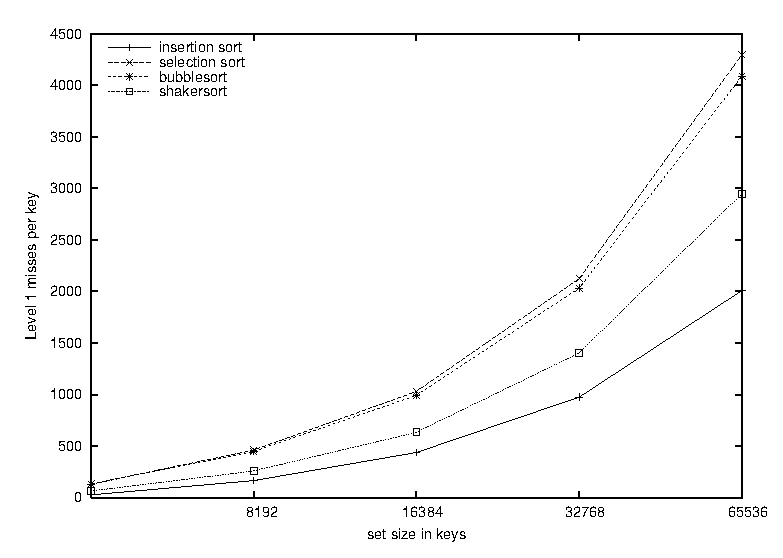
\includegraphics[scale=\myscale]{plots/on2_-_Level_1_misses.eps}}
\subfigure[Branches per key - this was simulated using \cc{sim-bpred}.]
{\label{elementary branches}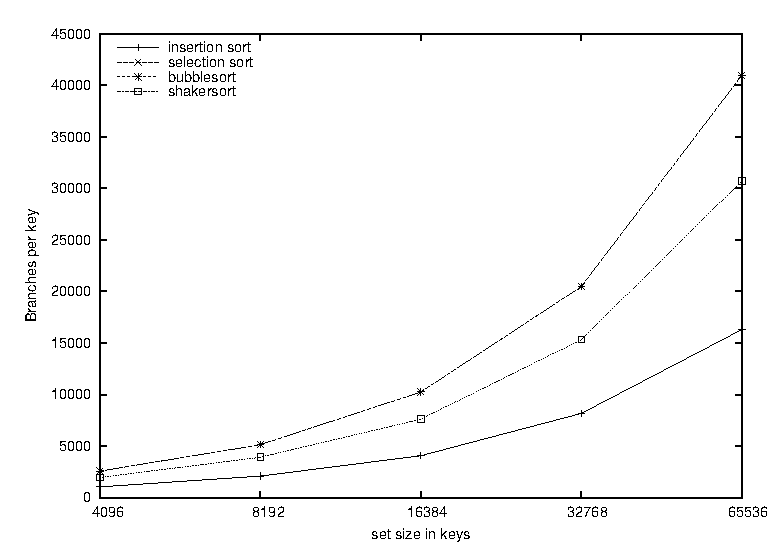
\includegraphics[scale=\myscale]{plots/on2_-_Branches.eps}}
\end{changemargin}
\vspace*{6em}
\caption{Cache and Branch prediction simulation results for elementary sorts}
\label{Cache and Branch prediction simulation results for elementary sorts}
\end{figure}
\newpage

\thispagestyle{empty}
\clearpage
\enlargethispage{14em}
\vspace*{-8em}
\begin{figure}[H]
\begin{changemargin}
\centering
\subfigure[Branches misses per key - this was simulated using \cc{sim-bpred}, with bimodal and two-level adaptive
predictors. The simulated two-level adaptive predictor used a 10 bit branch history register which was XOR-ed with the
program counter.]
{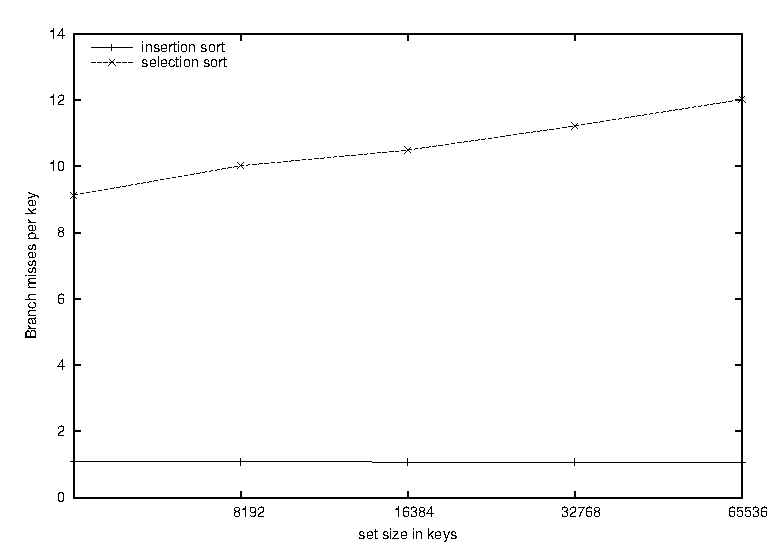
\includegraphics[scale=\myscale]{plots/on2_-_Branch_misses1.eps}}
\subfigure[Branches misses per key - this was simulated using \cc{sim-bpred}, with bimodal and two-level adaptive
predictors. The simulated two-level adaptive predictor used a 10 bit branch history register which was XOR-ed with the
program counter.]
{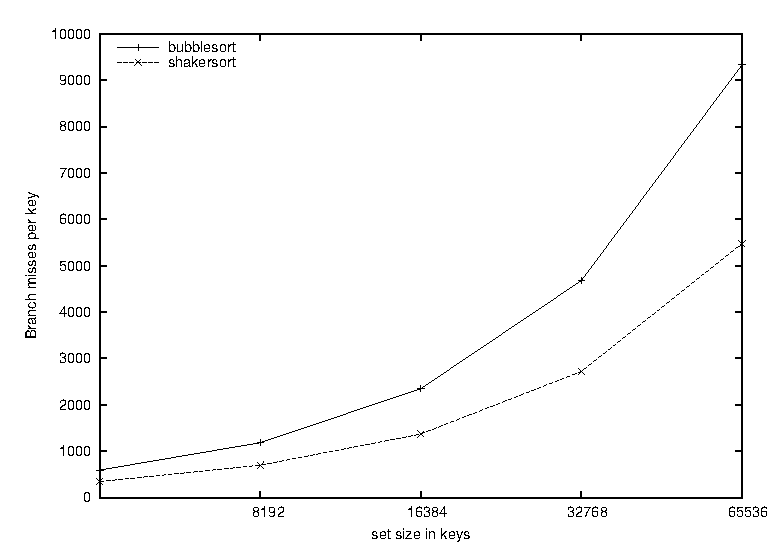
\includegraphics[scale=\myscale]{plots/on2_-_Branch_misses2.eps}}
\end{changemargin}
\vspace*{6em}
\caption{Branch Simulation results for elementary sorts}
\label{Branch Simulation results for elementary sorts}
\end{figure}
}

Figure \ref{elementary instructions} shows the instruction count of each
elementary sort. Each sort's instruction count is as predicted. Selection sort
has the most instructions, and insertion sort has approximately half that
number, as predicted. Bubblesort has almost the same number of instructions as
selection sort, but shakersort has a significant number less. The improvement to
bubblesort in improved bubblesort have increased the instruction count, contrary to
predictions, and similarly in the improved shakersort. It appears the cost of
skipping over a segment of the array is not worth the additional book-keeping
cost of determining when this can be done.

The level 2 cache performance of these sorts is not considered, as the set sizes
are never larger than the level 2 cache. Instead, the level 1 caches are used,
and their performance can be used to approximate the level 2 cache in these
cases. These results are shown in Figure \ref{elementary level 1 misses}. Each
set size is larger than the cache, and each sort iterates across the entire
array each time, leading to very poor performance.

As expected, selection sort has the worst cache performance. This is due to the
fact that it considers the entire unsorted segment of the array for each key to
be put in place. Bubblesort, with similar behaviour, is only slightly better.
Shakersort has a small amount of temporal reuse, reducing its number of misses.
Improved shakersort is placed roughly between insertion sort and shakersort,
showing that ending early is helpful in its case. This does not appear to be the
case with improved bubblesort though, which performs identically to bubblesort.

Insertion sort performs best of these sorts in relation to cache misses. This
is due to the fact that the keys it considered most recently are used again for
the next key. These keys will be swapped out fairly regularly, however, but not
nearly as often as selection sort, where they are swapped out at nearly every
iteration.

Figure \ref{elementary branches} shows the number of branches per key of these
sorts, while Figure \ref{Branch Simulation results for elementary sorts} shows
the branch misses per key. Due to huge variations in predictability, we split
the numbers of branch mispredictions into two charts. Selection sort causes
around $H_N$ mispredictions per key, which is remarkably small. The comparison
branch in the inner loop is highly predictable on random data, because a good
candidate minimum is usually found quickly.

Selection sort, meanwhile, has the same number of branches as bubblesort, but
only $O(H_N)$ misses per key. The most interesting result, though, is insertion
sort. This has exactly one miss per key. Although this result was not predicted
in advance, on reflection this behaviour is obvious: every iteration involves
moving the key left. The only time it will not move left is when its being put
into place, and this only happens once for every key. This shows that it is
possible to completely eliminate even comparative branch misses. It also
establishes insertion sort as the best of the simple sorts, and it is used later
in quicksort and mergesort as a result of this. \label{insertion is predictable}

The number of misses for bubblesort and shakersort are so huge that we had to
plot them on a separate chart. Nearly one in four comparisons are misses. As the
data sets gets large, there are nearly 10,000 branch misses involved in sorting
a single key. The improved bubblesort had exactly the same number of misses and
branches. The improved shakersort has a lot less branches, but the same number
of misses. This is because skipping over sorted keys is predictable from the
first branch miss.

The branch behaviour of bubble sort is particularly interesting when
compared to selection sort. Although we usually think of the two
algorithms as being different, they are actually very similar. Like
selection sort, bubble sort finds the smallest (or largest) key in the
unsorted part of the array and moves it to start (end) of the array.
Thus, we would expect that bubbble sort's branch prediction behaviour
would be similar to that of selection sort.

However, in the proces of moving the smallest element into position,
bubble sort also rearranges other array elements. Selection sort
sweeps across the array and always keeps track of the left-to-right
minimum up to the current point. However, bubble sort actually moves
this minimum, exchanging pairwise with each element it encounters
which is larger. Thus, even the unsorted part of the array becomes
partially sorted. We might expect that bubble sort's comparison branch
for a partially sorted array might be more predictable than for a
random one, but it is not. With a random array, the smaller elements
are equally likely to appear anywhere in the array. With a partially
sorted array, the smaller elements tend to appear towards the start of
the array which is, in bubble sort, the last place that we look. Thus,
we change the candidate minimum much more often than if we were
searching a randomly ordered array.



\section{Future Work}
Simulations from elementary sorts take a lot of time. Running the simulation for
bubblesort with 65536 keys takes nearly a day, and the simulation for 4194304
keys would take nearly 11 years to run. Due to this, it is necessary to
extrapolate results for larger data sets from the results from these smaller
sets. The only place where it's necessary to have larger data sets is in the
case of cache results. The cache behaviour of these sorts should change
dramatically once the keys no longer fit in the cache, as they do in subsequent
chapters with other sorts. The results can be simulated, by using a
smaller cache, but in this case all the data sets are too large. It would be
easy to use data sets smaller than the cache, but in this case many factors
would not have time to be amortised, such as filling the cache and branch
prediction tables.

Each of these sorts could have the number of iterations across the array reduced
by a half or a third by considering two or three keys at a time. The resultant
reduction in cache misses is predictable, and instruction count should reduce.
The new branch prediction results, especially in the case of insertion sort, may
be significantly worse, or may stay the same. The results of this would be
interesting.

It should be possible to make more cache-conscious versions of these sorts.
Making a bubblesort which performs a bubble across an entire cache line would
be an example. However, these would only make a difference on large data sets,
when better sorts such as quicksort should be used. In addition, the complexity
of doing this means it may be easier to code a simple $O(NlogN)$ sort, which
would perform better for the same effort. Due to this, a cache-conscious
elementary sort is but an academic exercise.
